\chapter{Metodología}\label{cap:metodologia}

El método final no fue el primero. Este capítulo cuenta primero cómo evolucionó (secciones~\ref{sec:idea-inicial}
a~\ref{sec:idea-tabroll}), porque cada cambio respondió a algo que mostró el audio. Después describe el algoritmo final
(sección~\ref{sec:algoritmo}), las decisiones sobre la melodía y la armonía, la evaluación y la comparación con estilos.

\section{La idea inicial y lo que mostró el audio}\label{sec:idea-inicial}

El trabajo partió de cuatro supuestos, y cada uno se puso a prueba contra el audio
(tabla~\ref{tab:supuestos}).

\begin{table}[ht]
  \centering\small
  \caption{Supuestos iniciales y cómo se pusieron a prueba.}\label{tab:supuestos}
  \begin{tabularx}{\textwidth}{@{}>{\raggedright}X>{\raggedright\arraybackslash}X@{}}
    \toprule
    Supuesto & Cómo se puso a prueba \\
    \midrule
    Los cuartos de tono solo aparecen en una zona del mástil: la parte más aguda como $\mathbb{Z}_{24}$ y el resto como
    $\mathbb{Z}_{12}$. & Medir cada nota sin decidir antes dónde puede haber cuartos de tono. \\
    La partitura publicada sirve como referencia principal para medir la precisión. & Escucharla frente a fragmentos de
    la grabación. \\
    Basta con pYIN para obtener la melodía. & Seguir con pYIN el bajo de Sarniezz. \\
    Las secciones de la canción se reconocen por el timbre. & Resumir el timbre de cada fragmento con MFCC y entrenar una
    red neuronal pequeña para reconocer la sección. \\
    \bottomrule
  \end{tabularx}
\end{table}

El primer supuesto se formalizó como una cuantización a trozos según el índice de traste $k$: los trastes de cuarto de
tono hasta una posición $k_0$ y de semitono a partir de ella,
\[
  f(k) =
  \begin{cases}
    f_0 \cdot 2^{k/24}, & k \le k_0, \\
    f(k_0) \cdot 2^{(k - k_0)/12}, & k > k_0,
  \end{cases}
\]
inspirada en el instrumento de Khn: la guitarra tiene 30 trastes de cuarto de tono seguidos de 6 de semitono, y el bajo,
24 de cuarto de tono seguidos de 6 de semitono. \pv[: número de trastes de cada instrumento] El método final no presupone
esa división: mide cada nota en la rejilla completa de 24-EDO.

El punto de partida fue la transcripción de Sarniezz en MuseScore, leída como piano roll en un primer cuaderno de Python
(figura~\ref{fig:primer-cuaderno}).

\begin{figure}[htbp]
  \centering
  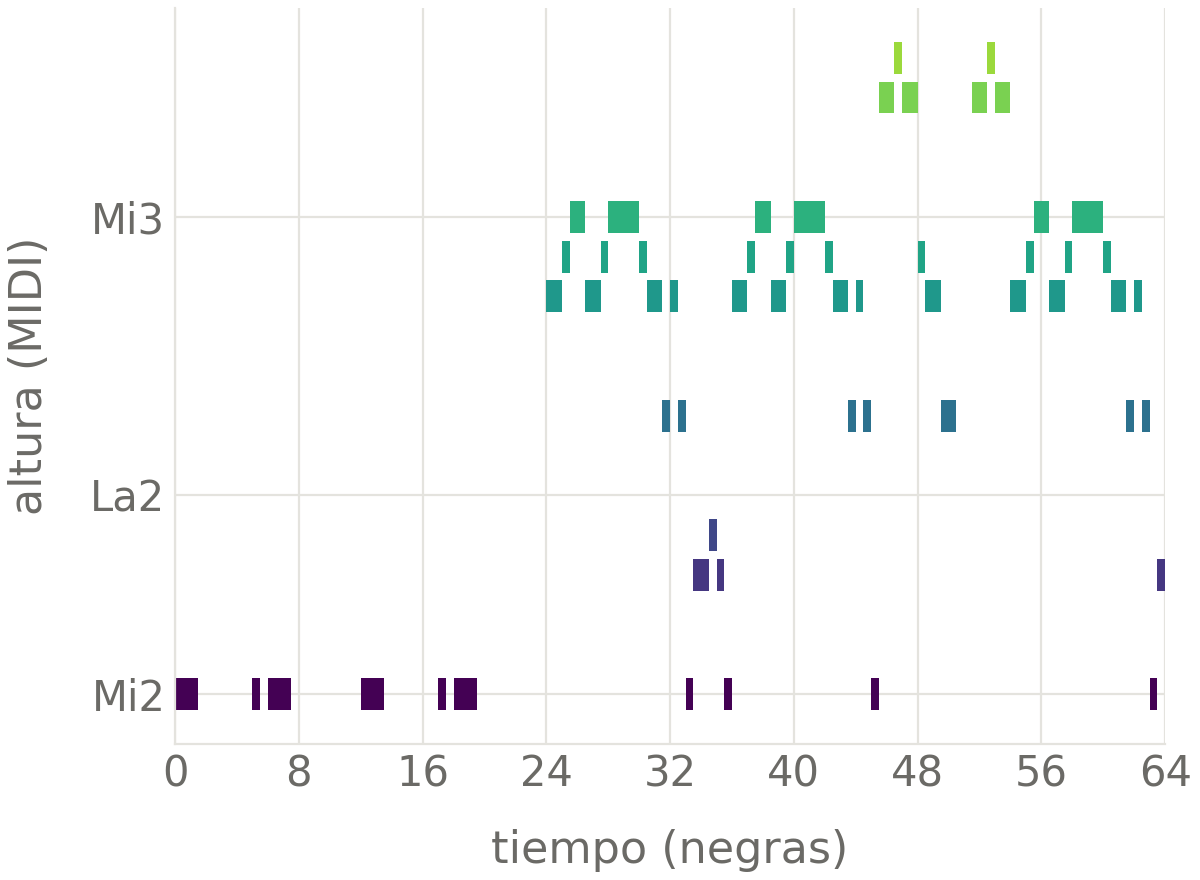
\includegraphics[width=0.75\textwidth]{cuaderno_original_sarniezz.png}
  \caption{Primer cuaderno: la partitura de Sarniezz en piano roll (primeras 64 negras). Aún no se medía el audio.}
  \label{fig:primer-cuaderno}
\end{figure}

\section{El primer algoritmo y por qué no bastó}\label{sec:primer-algoritmo}

El primer algoritmo tomó la pista de bajo de Sarniezz y le aplicó pYIN (de Do2 a Do7, ventana de 2048 muestras), que da
una altura por instante. Después midió la desviación en cents respecto del semitono más cercano. Por último, una red
neuronal intentó reconocer la sección de la canción a partir del timbre: 28 fragmentos del bajo de Sarniezz (27 de 10~s
y uno de 9.1~s), etiquetados a mano en seis secciones; 13 MFCC por fragmento, resumidos en su media y su desviación (26
números); un perceptrón de dos capas ocultas (64 y 32 neuronas) con partición estratificada de 21 fragmentos de
entrenamiento y 7 de prueba.

Las tres pruebas mostraron límites (figura~\ref{fig:primer-algoritmo}):
\begin{itemize}
  \item En el álbum suenan varias capas del looper al mismo tiempo, y pYIN, que solo ve una, salta de una a otra: no separa
  las voces ni da acordes.
  \item La desviación respecto del semitono más cercano siempre cae entre $-50$ y $+50$ cents. Un cuarto de tono queda
  justo en el borde y no se distingue de una nota desafinada.
  \item La red acertó 3 de 7 fragmentos (43\,\%). Con 21 ejemplos para seis secciones, y un timbre del bajo casi igual
  en toda la canción, los MFCC no bastan para reconocer la sección.
\end{itemize}

\begin{figure}[htbp]
  \centering
  \begin{subfigure}{\textwidth}\centering
    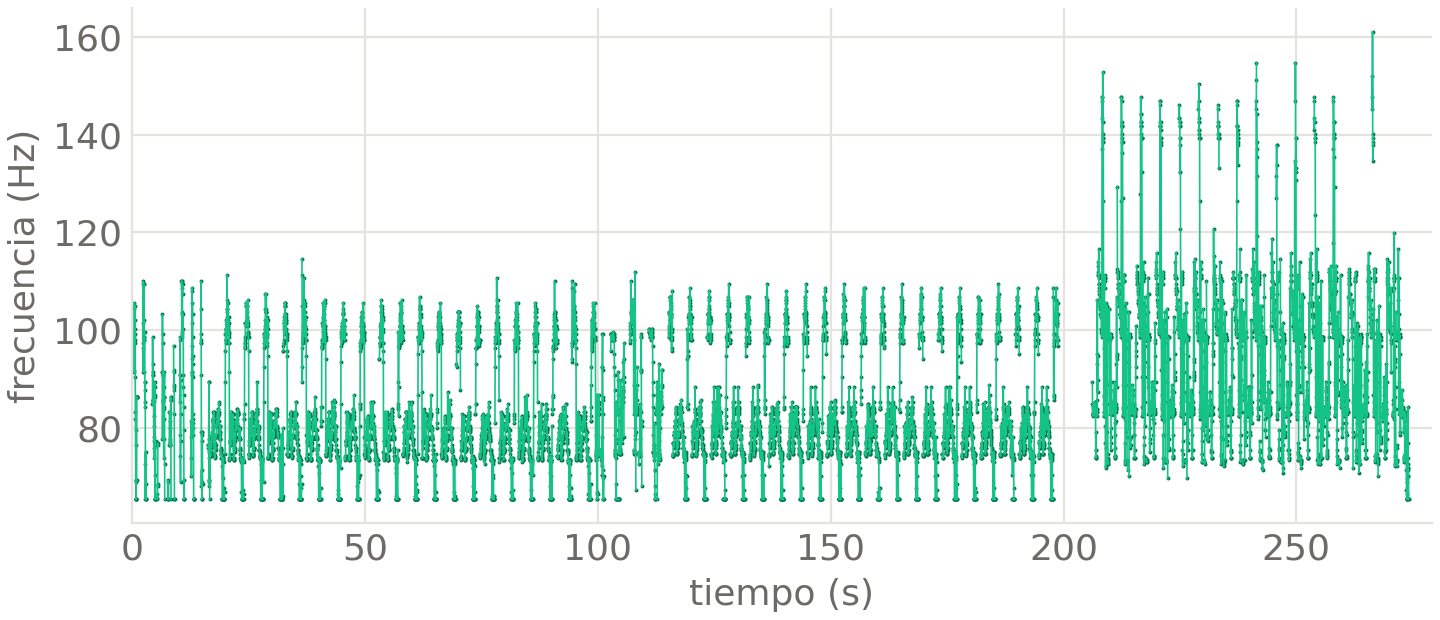
\includegraphics[width=0.8\linewidth]{original_pyin.png}
    \caption{pYIN da una sola altura por instante: no ve acordes.}
  \end{subfigure}\\[0.6em]
  \begin{subfigure}{0.6\textwidth}\centering
    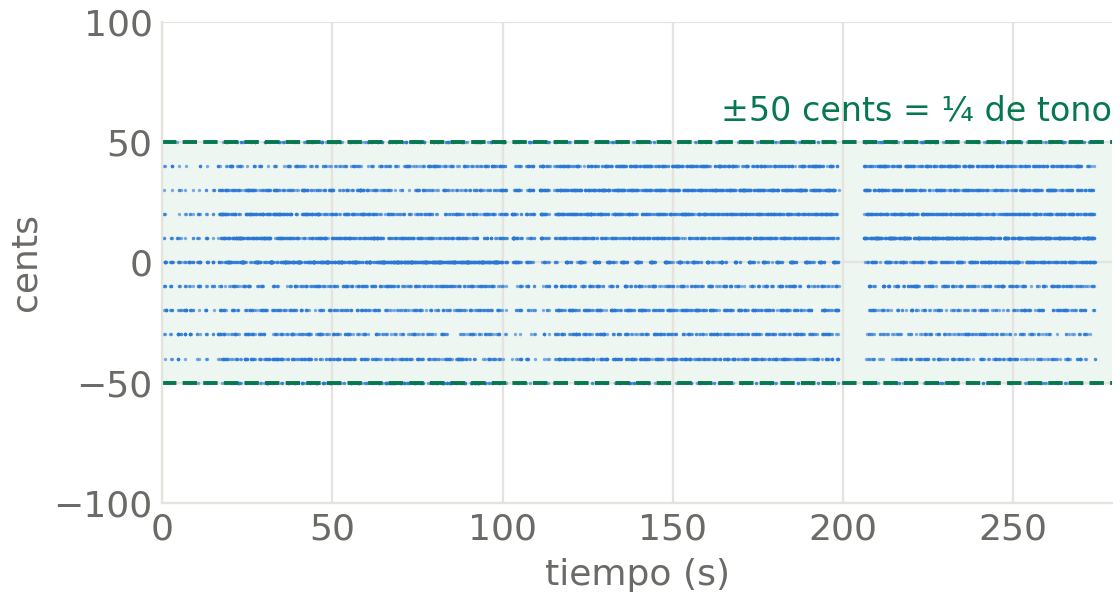
\includegraphics[width=\linewidth]{original_cents.png}
    \caption{La desviación del semitono nunca pasa de $\pm50$ cents: el cuarto de tono queda ambiguo.}
  \end{subfigure}\hfill
  \begin{subfigure}{0.36\textwidth}\centering
    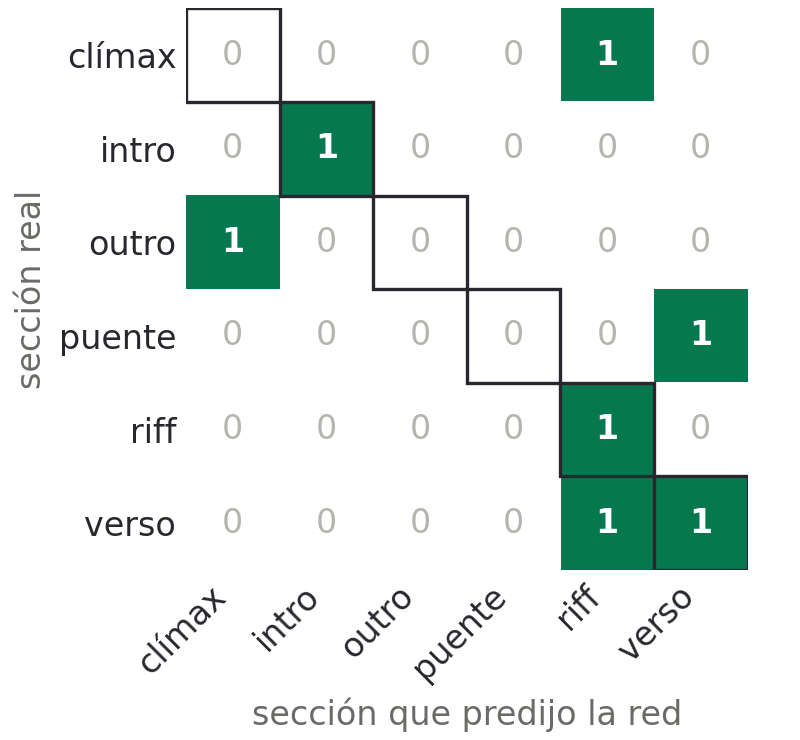
\includegraphics[width=\linewidth]{original_secciones_mlp.png}
    \caption{Matriz de confusión de la red por sección: acierta 3 de 7.}
  \end{subfigure}
  \caption{Primer algoritmo: por qué no bastó.}\label{fig:primer-algoritmo}
\end{figure}

Además, la partitura publicada resultó no ser un criterio fiable: también se equivoca, y la de Fabienk corresponde a la
versión en vivo. La conclusión fue que había que pasar de describir la señal a \emph{transcribir} notas, compases y
acordes, y que la referencia tenía que corregirse de oído.

El cuaderno empezó en Google Colab y pasó a un repositorio de GitHub cuando la memoria disponible dejó de alcanzar.

\section{La idea del tabroll}\label{sec:idea-tabroll}

Al estudiar la armonía de Primus se encontró el formato de Hooktheory \citep{hooktheory}: fragmentos de canciones transcritos a mano en un
piano roll dividido por compases, con la melodía arriba y el acorde de cada compás abajo. Hooktheory tiene una sola
canción de la banda, el riff de Fabienk, en doce notas por octava.

El \emph{tabroll} recrea esa idea con dos cambios: 24 filas por octava, para que los cuartos de tono tengan su lugar, y
generación automática desde el audio oficial de cualquier canción, sin transcribir nada a mano
(figura~\ref{fig:tabroll}). En el tramo de Fabienk de 4:42 a 4:52 (la melodía «Fabien»), la voz aguda del tabroll da la
misma nota que la partitura corregida el 78\,\% del tiempo, y 6 de sus 8 cuartos de tono están en la partitura.

\begin{figure}[htbp]
  \centering
  \begin{subfigure}{0.44\textwidth}\centering
    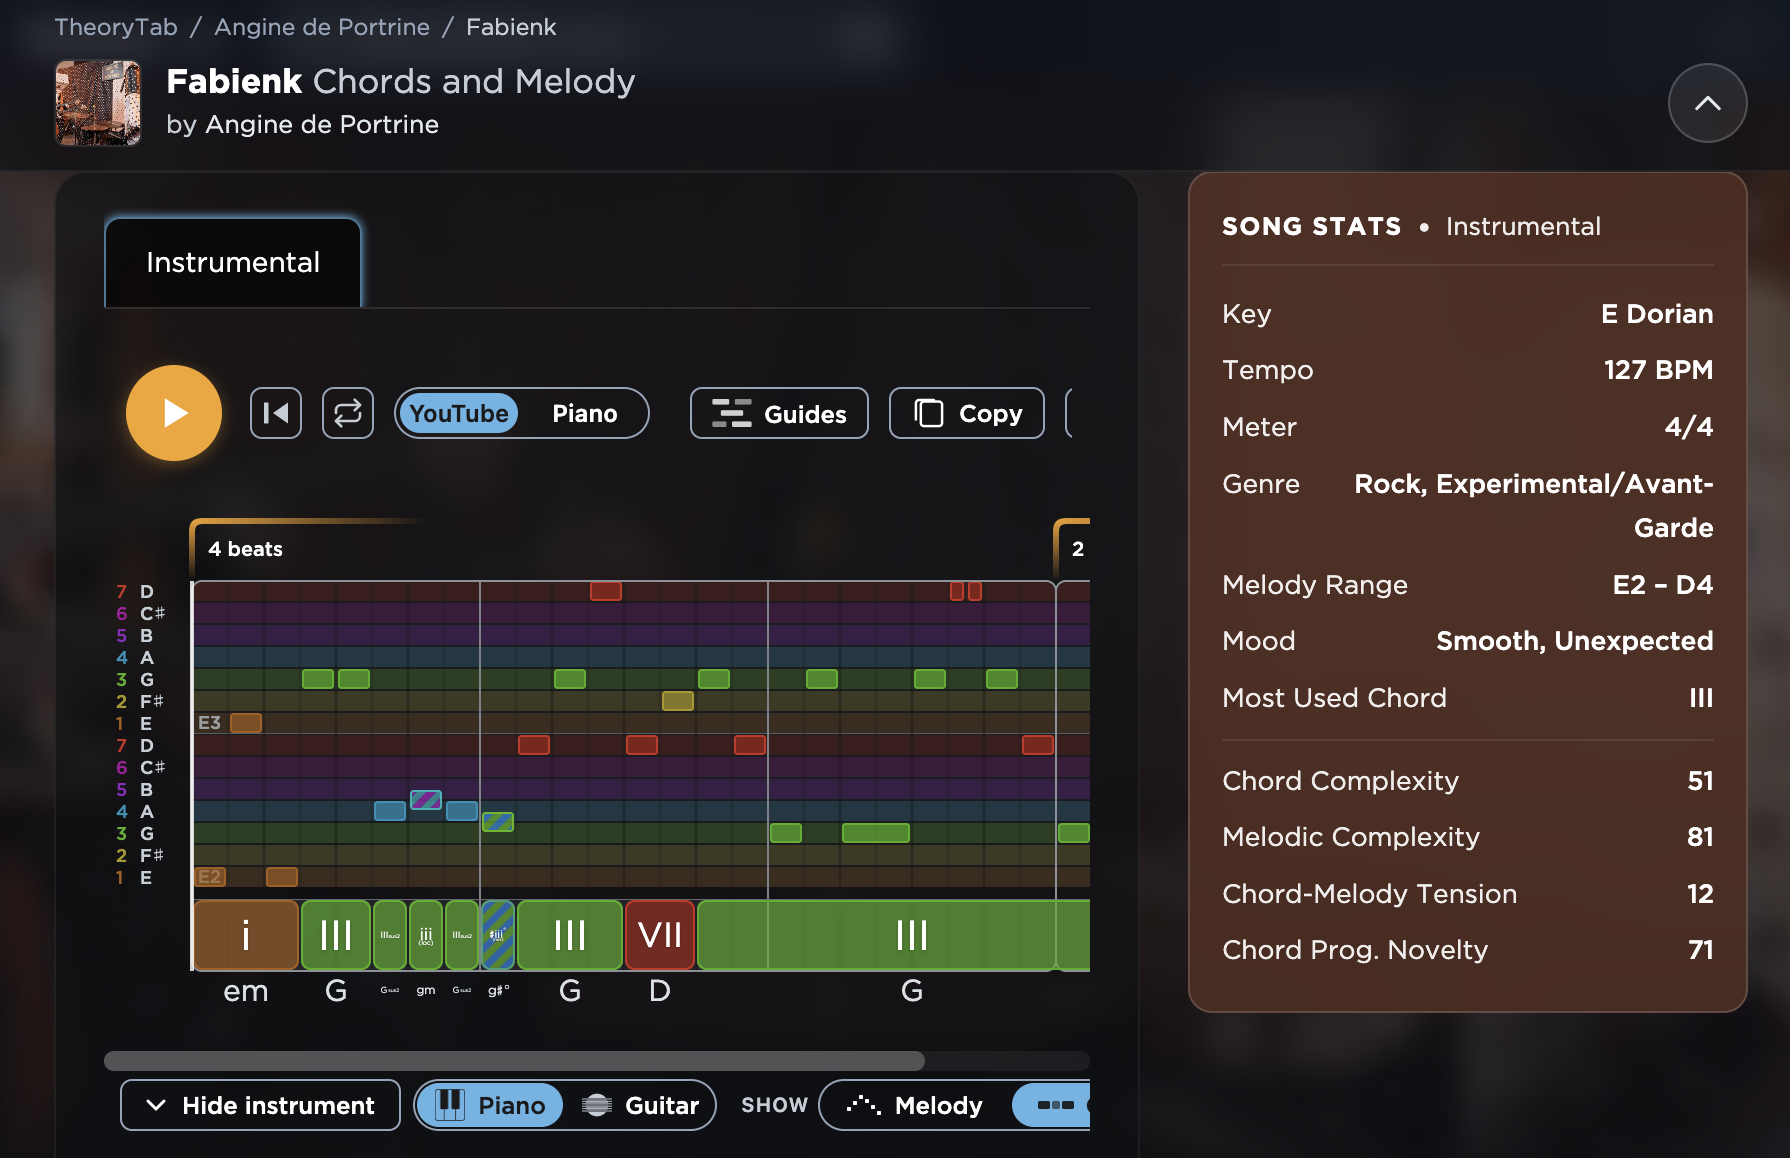
\includegraphics[width=\linewidth]{hooktheory_fabienk.png}
    \caption{Hooktheory (a mano): Mi dórico, 4/4, 12 notas.}
  \end{subfigure}\hfill
  \begin{subfigure}{0.53\textwidth}\centering
    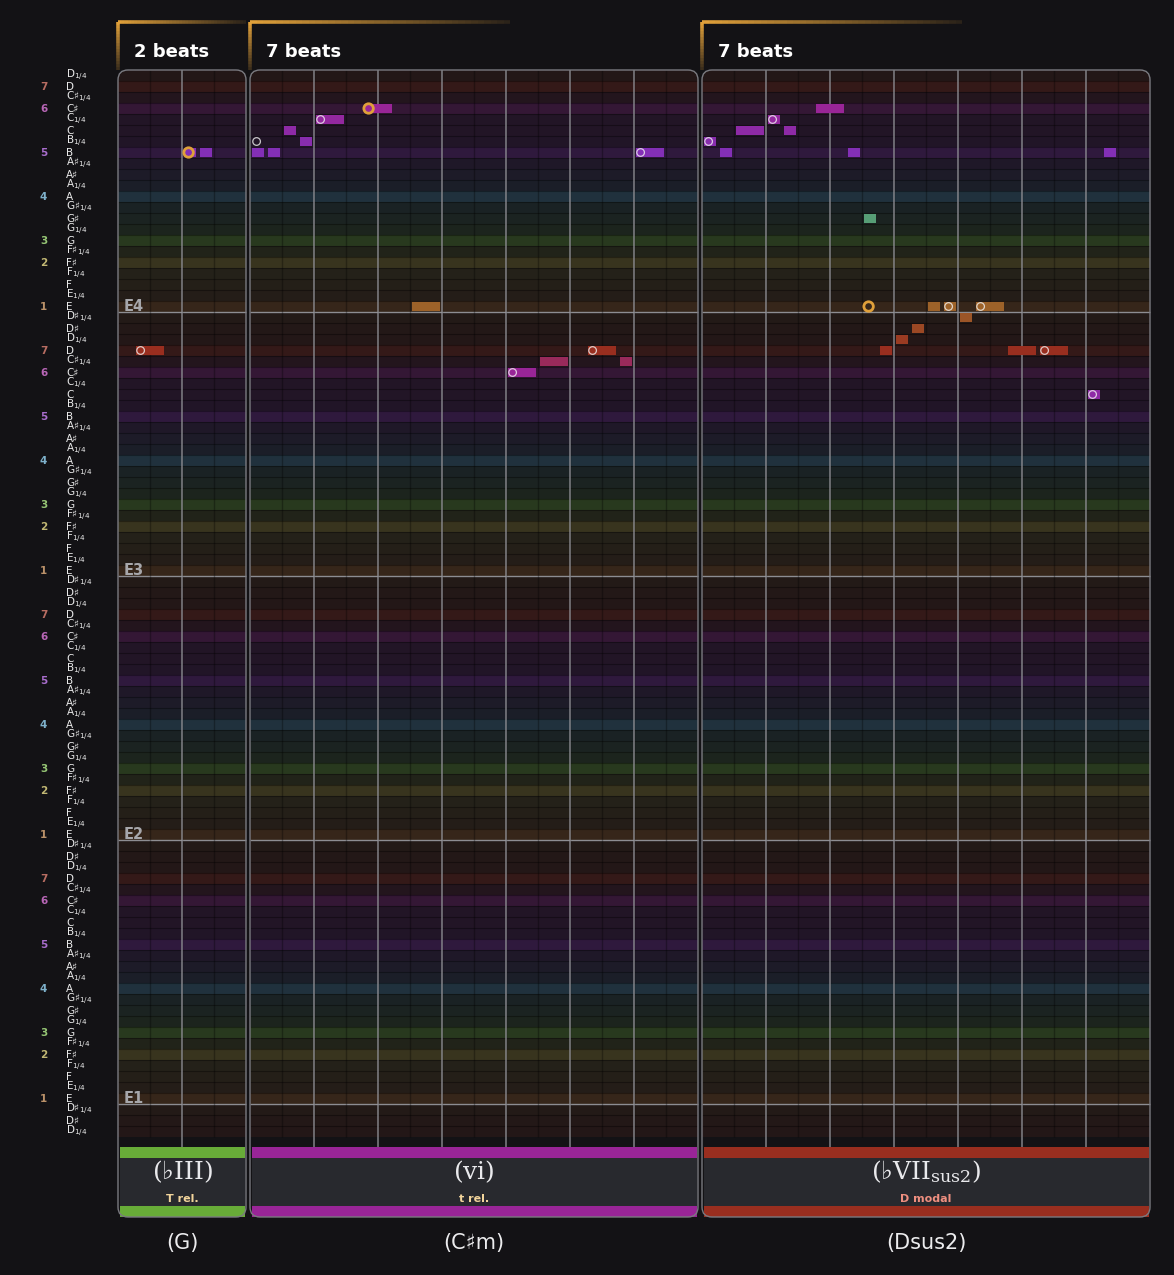
\includegraphics[width=\linewidth]{tabroll_fabienk.png}
    \caption{Tabroll desde el audio (4:42--4:52): los cuartos de tono, en las filas «+» azules.}
  \end{subfigure}
  \caption{De Hooktheory al tabroll: Fabienk en 12 notas y en 24.}\label{fig:tabroll}
\end{figure}

\section{Las primeras comparaciones con estilos}\label{sec:primeras-comparaciones}

La comparación con estilos también pasó por varias versiones antes del test por bloques.

\begin{enumerate}
  \item \textbf{Pop de Hooktheory.} La primera comparación fue con nueve álbumes de pop analizados en Hooktheory. La banda
  quedó lejos: a una distancia de Jensen-Shannon de 0.40 a 0.59, cuando los álbumes entre sí no pasan de 0.07.
  \item \textbf{Tarjetas al estilo de Hooktheory.} Las cinco métricas de Hooktheory son percentiles frente a su base de unas
  40\,000 canciones y no se pueden recalcular fuera de ella, así que se usaron valores crudos y las de Hooktheory solo
  como contexto. El resultado es una tarjeta por canción (figura~\ref{fig:tarjeta-mata}).
  \item \textbf{Pruebas de estilo con reglas.} Se definieron reglas con cifras publicadas para el rock, la práctica común,
  el jazz, la pentatónica, los tonos enteros, el dodecafonismo, el minimalismo y la música microtonal. Sirvieron para
  descartar: el jazz, la práctica común, los tonos enteros y el dodecafonismo no encajan en ninguna canción, y las
  fundamentales de la banda caen casi por completo en la pentatónica menor (del 86 al 100\,\% del tiempo). Pero los
  umbrales de las reglas los fijaba el autor, y eso era una debilidad. Los veredictos y las distancias de esta versión
  están en el apéndice (figuras~\ref{fig:g-distancias} a~\ref{fig:g-veredictos2}).
  \item \textbf{Matriz de verosimilitud.} Para no depender de umbrales propios, se pasó a ubicar cada canción dentro de la
  distribución real de cada estilo, con corpus: es la matriz de la sección~\ref{sec:comparacion}.
  \item \textbf{Radares.} Una figura de radar con una punta por estilo, separada en armonía, melodía y ritmo, resumía el
  perfil de cada canción (figura~\ref{fig:radar-mata}). La primera versión ponía cada punta en su propia escala, lo que
  impedía comparar puntas; se corrigió usando la verosimilitud.
  \item \textbf{Test por bloques.} Finalmente, la comparación se separó en bloques y se calibró con el error medido en
  Primus (sección~\ref{sec:comparacion}).
\end{enumerate}

\begin{figure}[htbp]
  \centering
  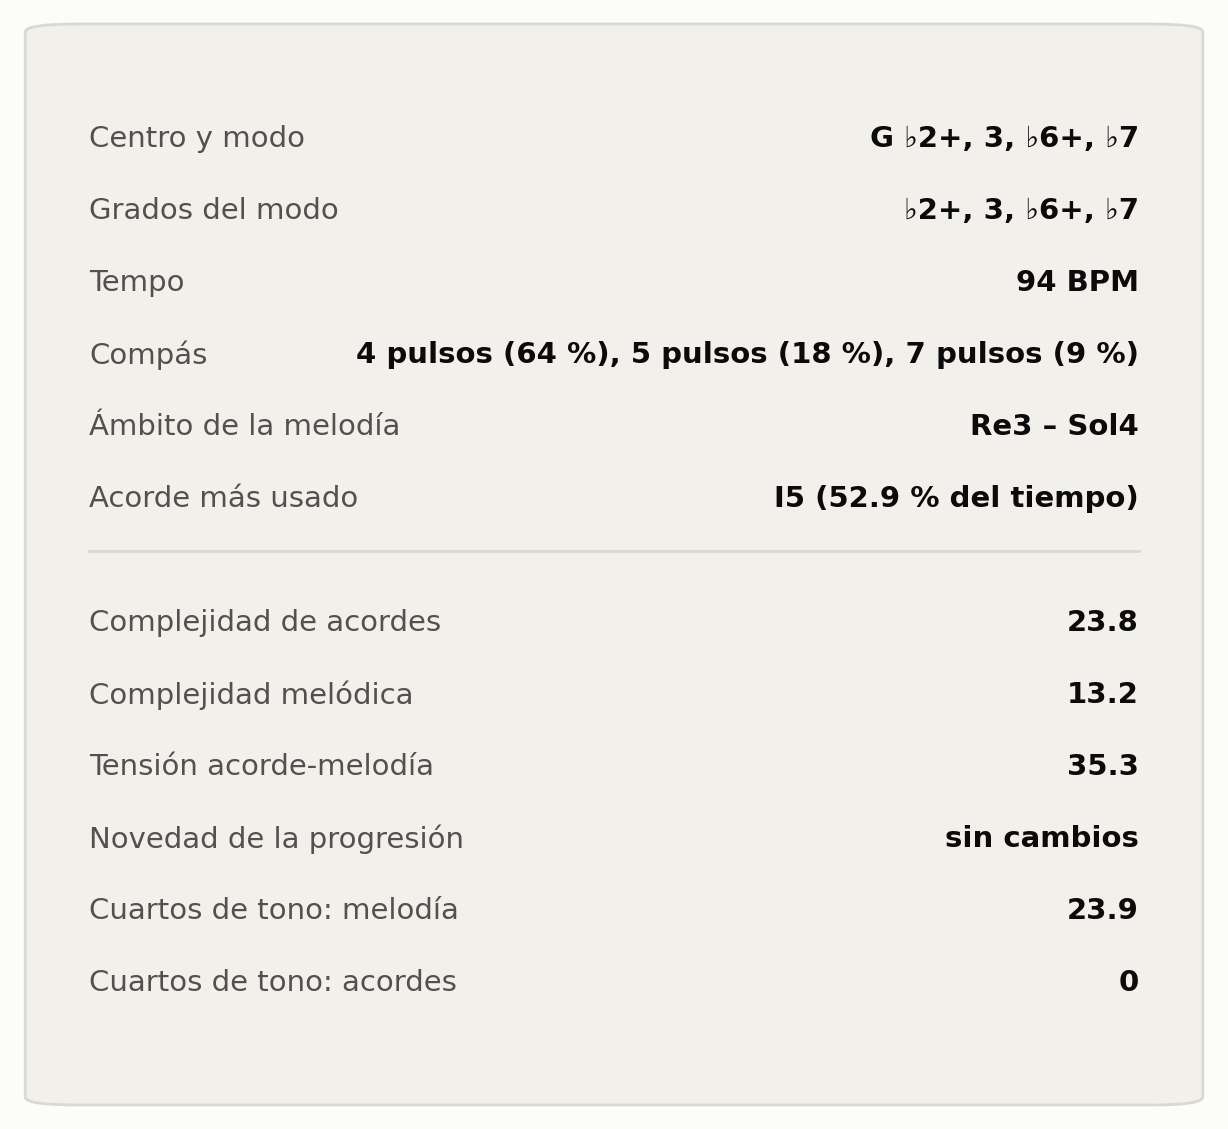
\includegraphics[width=0.5\textwidth]{mata_zyklek_tarjeta.png}
  \caption{Tarjeta de Mata Zyklek. Arriba, centro, modo, tempo, compases, ámbito y acorde más usado; abajo, seis métricas en valores crudos (0--100 o \% del tiempo; no son percentiles). Compases confiables: 78.3\,\% del tiempo; acierto contra la referencia: F 66.5 en la melodía y 95.4 en la fundamental.}\label{fig:tarjeta-mata}
\end{figure}

\begin{figure}[htbp]
  \centering
  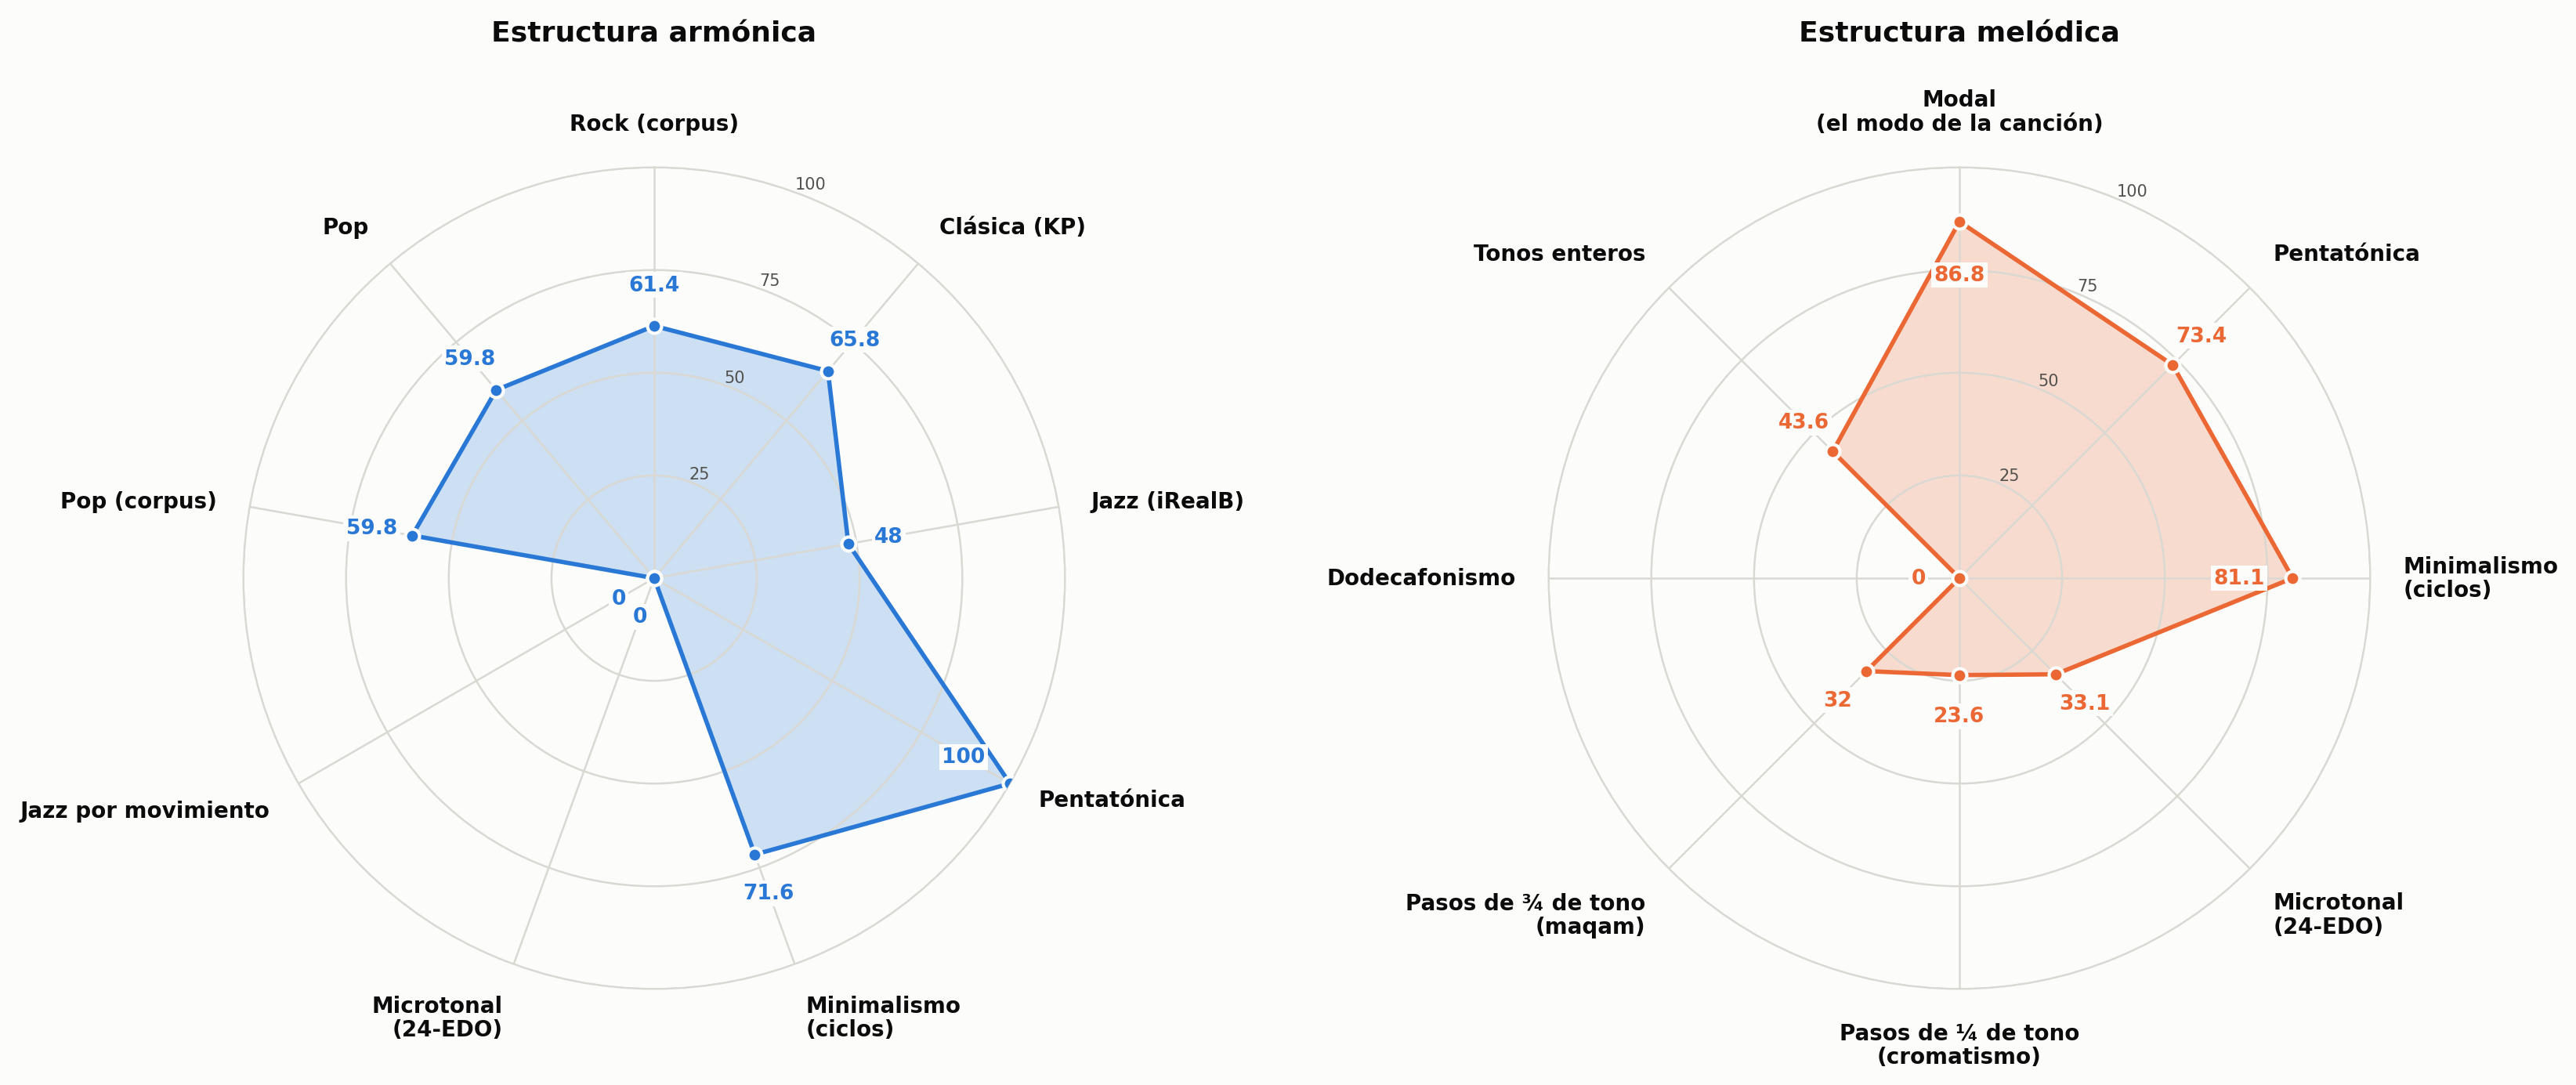
\includegraphics[width=\textwidth]{mata_zyklek_radar_estilos.png}
  \caption{Radar de estilos de Mata Zyklek (versión descartada, 15 de noviembre). Izquierda: armonía; derecha: melodía. Cada punta es un estilo en escala de 0 a 100: más lejos del centro, más parecido.}\label{fig:radar-mata}
\end{figure}

También la lectura de los cuartos de tono cambió. La primera versión medía solo la \emph{cantidad} de tiempo en cuartos
de tono, y la banda salía con poca microtonalidad, porque las fundamentales de los acordes casi nunca caen en cuarto de
tono. Después se intentó separar adorno de grado por la duración de la nota, pero Primus también daba «grados». Lo que sí
separa a la banda del control es la \emph{concentración} en pocos grados fijos (sección~\ref{sec:metodo-cuartos}).

\section{El algoritmo completo}\label{sec:algoritmo}

El algoritmo final tiene tres etapas (algoritmo~\ref{alg:tabroll}). La primera prepara la señal. La segunda, el núcleo
propio del trabajo, transcribe en 24-EDO guiada por el looper: como la banda repite cada riff, la altura se promedia entre
vueltas antes de decidir la nota, y por eso el método funciona con cuartos de tono. La tercera extrae la estructura y
compara con los estilos. La tabla~\ref{tab:parametros} da los parámetros, que vienen del código.

\begin{algorithm}[ht]
  \caption{TabRoll24($x$): del audio al veredicto de estilo.}\label{alg:tabroll}
  \KwIn{audio estéreo $x$}
  \KwOut{notas $N$ en 24-EDO, compases $B$, acordes $A$ y veredicto $V$ por bloque}
  \tcp{1 · Señal}
  $(g, b) \leftarrow \textsc{Separar}(x)$\tcp*{Demucs 6s, semilla 0}
  $S \leftarrow \textsc{Saliencia}(g, b)$\tcp*{10 armónicos, cada 25 cents}
  \tcp{2 · Núcleo: guiado por el looper}
  $\ell^* \leftarrow \textsc{Ciclo}(S)$\tcp*{autocorrelación, 1 a 16 s}
  $\hat S \leftarrow \textsc{Consenso}(S, \ell^*)$\tcp*{media en $\pm3$ vueltas}
  $w \leftarrow \textsc{Registro}(\hat S)$\tcp*{altura típica de la melodía}
  $m^* \leftarrow \textsc{Viterbi}(w \hat S)$\tcp*{contorno sin saltos innecesarios}
  $N \leftarrow \textsc{Notas}(m^*)$\tcp*{redondeo a \cuarto{} de tono}
  $N \leftarrow \textsc{Limpiar}(N, \ell^*)$\tcp*{fuera notas sueltas}
  \tcp{3 · Estructura y estilo}
  $B \leftarrow \textsc{Compases}(\textsc{Pulso}(x))$\tcp*{de 2 a 8 pulsos}
  \ForEach{compás $c \in B$}{
    $A[c],\ \kappa_c \leftarrow \textsc{Acorde}(c)$\tcp*{Piston y confianza}
  }
  \ForEach{bloque $\beta$, corpus $C$}{
    $\mathrm{pct}[\beta, C] \leftarrow \textsc{Percentil}(\beta, C)$\tcp*{5.ª vecina, $D_{\mathrm{JS}}$}
  }
  $V[\beta] \leftarrow$ «sin vecino» \textbf{si} $\max_C \mathrm{pct}[\beta, C] < 5$\;
  \Return{$N, B, A, V$}
\end{algorithm}

\begin{table}[ht]
  \centering\small
  \caption{Parámetros del algoritmo.}\label{tab:parametros}
  \begin{tabularx}{\textwidth}{@{}l>{\raggedright\arraybackslash}X@{}}
    \toprule
    Paso & Parámetros \\
    \midrule
    Separación & Demucs \texttt{htdemucs\_6s}, semilla 0 \\
    Saliencia & $H = 10$ armónicos, peso $0.82^{h-1}$, candidatas cada 25 cents \\
    Ciclos & autocorrelación, periodos de 1 a 16 s \\
    Consenso & media de la misma fase en $\pm3$ vueltas (ciclos de al menos 2 s) \\
    Registro & $w(m) = 0.7 + 0.3 \exp\!\bigl(-\tfrac12 ((m - r)/12)^2\bigr)$, con $r$ la mediana del contorno de base \\
    Viterbi & penalización de 0.01 por paso de 25 cents \\
    Notas sueltas & menos de 80 ms y sin repetición a $\pm1$ vuelta \\
    Compases & programación dinámica, longitudes de 2 a 8 pulsos \\
    Acorde & 8 calidades en 24-EDO; bajo con peso 1 y voz aguda con 0.6;
      $\kappa = p(\text{fundamental}) \cdot \text{acuerdo} \cdot \text{cobertura}$ \\
    Test & $k = 5$ vecinos (Jensen-Shannon), umbral de 5\,\%, error medido en Primus \\
    \bottomrule
  \end{tabularx}
\end{table}

\section{Cada paso en detalle}\label{sec:pasos}

Esta sección describe cada celda del cuaderno con su ecuación. El audio se analiza a $f_s = 22\,050$~Hz, con ventanas de
$N = 4096$ muestras (186~ms) y saltos de $H = 512$ muestras (23.2~ms): cada «cuadro» de las descripciones siguientes dura
23.2~ms.

\subsection{Espectro armónico}

La batería ensucia la estimación de altura: un golpe ocupa muchas frecuencias a la vez durante un instante, mientras que
una nota ocupa pocas frecuencias durante un rato. La celda \texttt{harmonic\_part} aprovecha esa diferencia con dos filtros
de mediana sobre el espectrograma $M$: uno a lo largo del tiempo ($\tilde H$, que conserva lo que se sostiene) y otro a lo
largo de la frecuencia ($\tilde P$, que conserva los golpes). La parte armónica es
\[
  M_{\mathrm{arm}} = M \cdot \frac{\tilde H^2}{\tilde H^2 + \tilde P^2},
\]
una máscara suave entre 0 y 1. Además, como el bajo suele ir al centro de la mezcla estéreo, el canal lateral
$\tfrac12(L - R)$ lo cancela; la saliencia de la voz aguda combina la mezcla, ese canal lateral y la pista de guitarra de
Demucs (\texttt{stereo\_salience}, \texttt{add\_guitar\_stem}).

\subsection{Saliencia}

La celda \texttt{pitch\_salience} comprime el espectro con $L = \log(1 + 20 M)$ y le resta su media local en frecuencia
(48 bandas), para que cuenten los picos y no el nivel general. Sobre ese espectro blanqueado $W$ calcula, para cada altura
candidata $p$ (de MIDI 26 a 100, cada 25 cents),
\[
  \Sigma(t, p) = \sum_{h=1}^{10} 0.82^{\,h-1}\, W\bigl(t,\, h f_p\bigr) \;-\; \gamma\, g(p) \min\bigl\{W(t, \tfrac12 f_p),
  W(t, \tfrac32 f_p)\bigr\},
\]
con $g(p)$ la suma de los pesos de los armónicos disponibles. El segundo término resta la huella de una nota una octava
más grave: si suenan $\tfrac12 f_p$ y $\tfrac32 f_p$, lo más probable es que $f_p$ sea el segundo armónico de esa nota y no
una nota propia. Con $\gamma = 0.7$ la saliencia elige la octava de la nota; con $\gamma = 0$ conserva la octava de la
guitarra, que es la que se usa para las notas del tabroll.

\subsection{Ciclos del looper}\label{sec:met-ciclos}

La celda \texttt{find\_cycles} busca los periodos que se repiten en una voz. Primero lleva el contorno a una sucesión de
clases $x_t$ (cada medio semitono) y, en ventanas de 30~s que avanzan de 5 en 5~s, calcula la autocorrelación de las
indicadoras de clase:
\[
  A(\ell) = \frac{\sum_c \sum_t \mathbf{1}[x_t = c]\, \mathbf{1}[x_{t+\ell} = c]}{\sum_t \mathbf{1}[x_t \text{ sonando}]\,
  \mathbf{1}[x_{t+\ell} \text{ sonando}]},
\]
que es la fracción de cuadros que suenan igual $\ell$ cuadros después. Los picos de $A$ entre 1 y 16~s que se repiten en
al menos dos ventanas son los periodos candidatos. Cada cuadro de la canción se asigna al periodo con mejor puntaje local,
y los tramos seguidos con el mismo periodo forman un \emph{ciclo}. Los ciclos con las mismas notas reciben la misma letra
(A, B, C\dots), lo que produce el mapa de ciclos de cada canción (capítulo~\ref{cap:resultados}).

La figura~\ref{fig:patron-ciclo} muestra dos de esos patrones en Mata Zyklek: la vuelta A de la voz aguda, de 10 pulsos,
y la vuelta A del bajo, de 5. Cada fila es un grado en 24-EDO y cada rectángulo, una nota del patrón consensuado entre
vueltas. La figura~\ref{fig:tira-mata} resume, para la misma canción, qué acordes trae cada ciclo y cuántas veces se
repite.

\begin{figure}[htbp]
  \centering
  \begin{subfigure}[b]{0.6\textwidth}\centering
    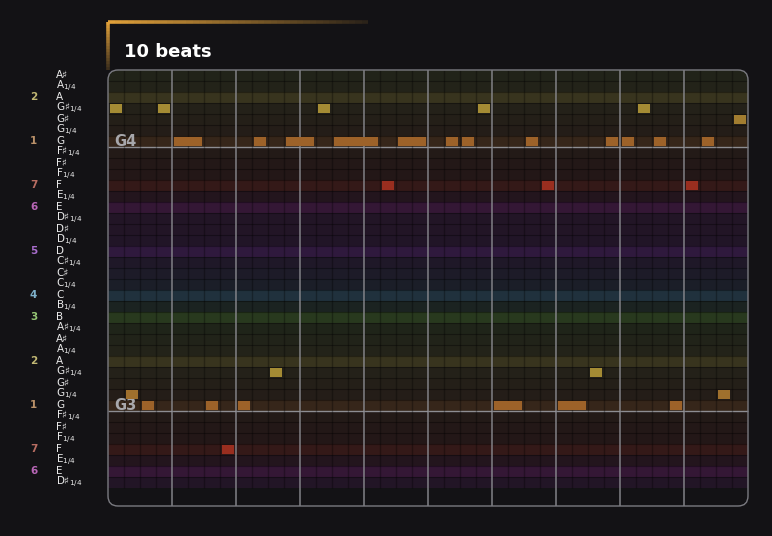
\includegraphics[width=\linewidth]{g_ciclo_aguda_mata.png}\caption{Voz aguda, ciclo A (10 pulsos).}
  \end{subfigure}\hfill
  \begin{subfigure}[b]{0.37\textwidth}\centering
    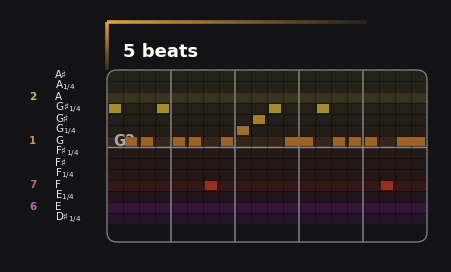
\includegraphics[width=\linewidth]{g_ciclo_grave_mata.png}\caption{Bajo, ciclo A (5 pulsos).}
  \end{subfigure}
  \caption{Patrones de ciclo de Mata Zyklek en 24-EDO. Cada fila es un grado y cada rectángulo, una nota que se repite en todas las vueltas. «Beats»: pulsos.}\label{fig:patron-ciclo}
\end{figure}

\begin{figure}[htbp]
  \centering
  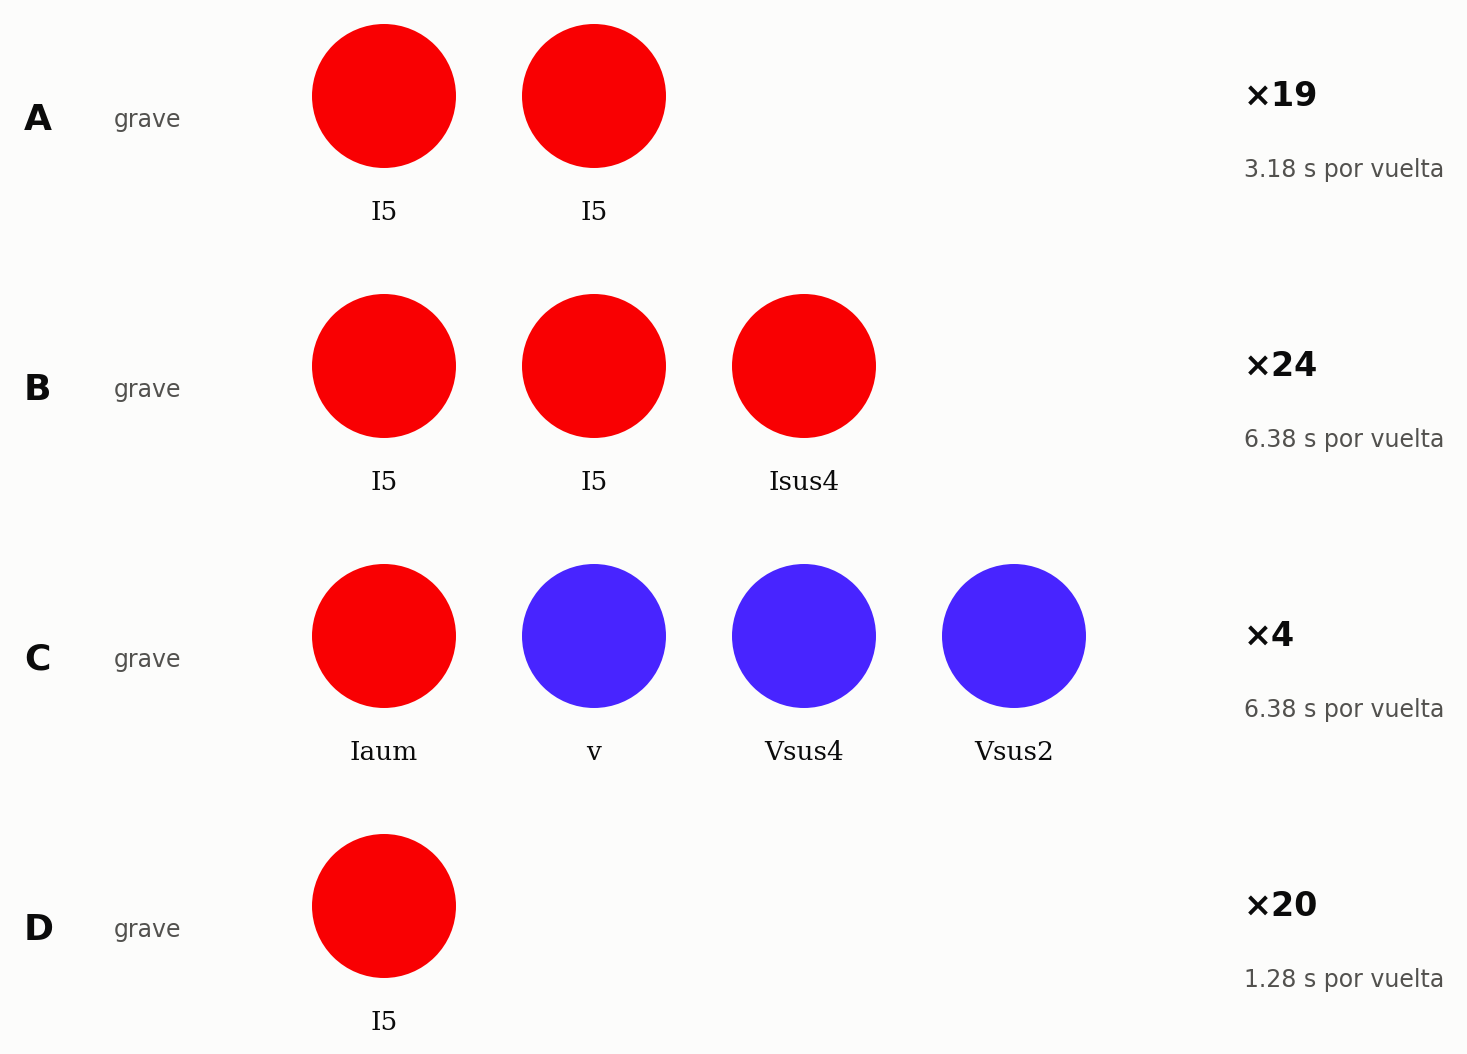
\includegraphics[width=0.75\textwidth]{mata_zyklek_tira_de_ciclos.png}
  \caption{Tira de ciclos de Mata Zyklek (centro Sol; modo \fl2+, 3, \fl6+, \fl7). Cada fila es un ciclo; cada círculo, la fundamental de un compás, con el color de su grado. A la derecha, número de vueltas ($\times$) y duración de cada vuelta.}\label{fig:tira-mata}
\end{figure}

\subsection{Consenso entre vueltas y atracción al registro}\label{sec:met-consenso}

Dentro de un ciclo de periodo $P \ge 2$~s, la saliencia de cada cuadro se reemplaza por su promedio con los cuadros
equivalentes de hasta tres vueltas antes y tres después:
\[
  \hat\Sigma(t, p) = \frac{1}{|K_t|} \sum_{k \in K_t} \Sigma(t + kP, p), \qquad
  K_t = \{k \in \{-3, \dots, 3\} : t + kP \text{ está en el ciclo}\},
\]
siempre que $|K_t| \ge 3$. Un error de una vuelta queda diluido entre las demás; una nota que se repite en todas las
vueltas se refuerza. Este es el paso que hace posible leer cuartos de tono: sin él, un cuarto de tono aislado no se
distingue de una nota desafinada.

Después se calcula un contorno de base con Viterbi sobre $\hat\Sigma$, se toma su mediana $r$ como el registro típico de la
melodía en la canción y se multiplica la saliencia por una atracción suave hacia ese registro:
\[
  w(p) = 0.7 + 0.3 \exp\!\Bigl(-\tfrac12 \bigl(\tfrac{p - r}{12}\bigr)^2\Bigr).
\]
La atracción nunca baja de 0.7, así que no impide salir del registro; solo desempata a favor de la zona donde suele estar
la melodía y en contra de los armónicos agudos o del bajo doblado.

\subsection{Contorno, notas y limpieza}

El contorno final es el camino de Viterbi sobre $w \hat\Sigma$ (proposición~\ref{prop:viterbi}). La celda
\texttt{extract\_notes} lo convierte en notas: cuantiza la altura a la rejilla de 50 cents, corrigiendo la desafinación
global de la grabación respecto de La 440 (\texttt{tuning\_offset}); aplica un filtro de mediana de tres cuadros; y corta
una nota nueva en cada ataque detectado y en cada cambio de altura. La altura de cada nota es la mediana del contorno en su
duración. Finalmente, \texttt{drop\_loose\_notes} quita las notas de menos de 80~ms que no reaparecen, con $\pm75$~ms de
tolerancia, a la misma altura una vuelta antes y una vuelta después.

\subsection{Tempo, pulso y compases}\label{sec:met-compases}

\paragraph{Tempo.} La celda \texttt{estimate\_tempo} calcula la autocorrelación $a(\ell)$ de la envolvente de ataques y,
para cada tempo candidato entre 60 y 200 BPM, con periodo $\ell(b)$, el puntaje
\[
  s(b) = \Bigl[a(\ell) + \tfrac12 a(2\ell) + \tfrac14 a(4\ell)\Bigr] \exp\!\Bigl(-\tfrac12 \bigl(\tfrac{\log_2(b/120)}{0.8}
  \bigr)^2\Bigr),
\]
que suma la evidencia del pulso y de sus múltiplos y prefiere suavemente los tempos cercanos a 120 BPM.

\paragraph{Pulso.} \texttt{track\_beats} aplica la programación dinámica de \citet{ellis2007} (sección~\ref{sec:senal}) con
rigidez $\alpha = 400$.

\paragraph{Evidencia de inicio de compás.} En cada pulso $i$ se combinan, estandarizados, el golpe grave, el golpe general
y el cambio de contenido armónico respecto del pulso anterior:
\[
  e_i = z\bigl(o^{\mathrm{grave}}_i\bigr) + 0.5\, z\bigl(o_i\bigr) + 0.8\, z\bigl(1 - \cos(h_{i-1}, h_i)\bigr),
\]
donde $h_i$ es el perfil de alturas del pulso. Además, \texttt{meter\_cue} mide, para cada longitud $L$, la correlación
$\rho_L(i)$ entre los ataques alrededor del pulso $i$ y los de $L$ pulsos después.

\paragraph{Segmentación.} \texttt{segment\_bars} elige la división en compases $L_1, L_2, \dots$, con cada $L_k$ entre 2 y
8 pulsos, que maximiza
\[
  \sum_k \Bigl[ e_{s_k} + \log \pi(L_k) + L_k\, \rho_{L_k}(s_k) \Bigr] - 0.8\, \#\{k : L_k \ne L_{k-1}\},
\]
donde $s_k$ es el pulso en que empieza el compás $k$ y $\pi$ es una distribución previa de longitudes (4: 0.45; 7: 0.15;
3: 0.12; 2, 6 y 8: 0.08; 5: 0.06). El último término penaliza cambiar de compás. Es un problema de Viterbi sobre los
estados «compás de longitud $L$ que termina en el pulso $j$», y se resuelve con la proposición~\ref{prop:viterbi}.

\subsection{Perfiles por compás y acorde}

\paragraph{Perfiles.} Para cada compás se calcula el tiempo que suena cada una de las 24 clases en el bajo, $P^b$, y en la
voz aguda, $P^m$ (sin las notas de menos de un cuarto de pulso). \texttt{fold\_bar\_profiles} los suma sobre todas las
vueltas del ciclo que contiene al compás y mide el \emph{acuerdo} entre vueltas como el coseno medio entre el perfil de
cada vuelta y el perfil sumado.

\paragraph{Acorde.} Con $b = P^b / \|P^b\|_1$ y $m = P^m / \|P^m\|_1$, la celda \texttt{chord24} forma el perfil combinado
$C = (b + 0.6\, m) / \|b + 0.6\, m\|_1$ y, para cada fundamental $r \in \mathbb{Z}_{24}$ y cada calidad $q$ con conjunto de
intervalos $I_q$ (tabla~\ref{tab:calidades}), el puntaje
\[
  S(r, q) = (1 + \lambda) \sum_{i \in I_q} C_{r+i} - \lambda + \beta\, b_r - \gamma \bigl(|I_q| - 2\bigr),
\]
con $\lambda = 0.5$, $\beta = 0.5$ y $\gamma = 0.02$. El primer término premia lo que cae dentro del acorde y, como
$\sum_i C_i = 1$, equivale a restar $\lambda$ veces lo que cae fuera; el segundo premia que el bajo esté en la
fundamental; el tercero penaliza levemente los acordes con más notas, para preferir la quinta sola cuando la tercera no
suena. Se elige el par $(r^*, q^*)$ de mayor puntaje. La probabilidad de la fundamental es un softmax con temperatura
$\tau = 0.05$ sobre los mejores puntajes de cada fundamental:
\[
  p(r^*) = \frac{\exp\bigl(\max_q S(r^*, q)/\tau\bigr)}{\sum_{r} \exp\bigl(\max_q S(r, q)/\tau\bigr)}.
\]

\begin{ejemplo}
Sea un compás con el bajo siempre en Mi ($b_{\mathrm{Mi}} = 1$) y la voz aguda repartida por igual entre Mi, Sol y Si. Con
Mi en la clase 8, Sol en la 14 y Si en la 22, se tiene $C = (b + 0.6\, m)/1.6$, es decir, $C_8 = (1 + 0.2)/1.6 = 0.75$ y
$C_{14} = C_{22} = 0.2/1.6 = 0.125$. Para la fundamental Mi y la calidad m ($I = \{0, 6, 14\}$, que sobre Mi da las clases
8, 14 y 22), $S = 1.5 \cdot 1 - 0.5 + 0.5 \cdot 1 - 0.02 = 1.48$. Para la calidad 5 ($I = \{0, 14\}$), el ajuste solo
cubre $0.875$ y $S = 1.5 \cdot 0.875 - 0.5 + 0.5 = 1.3125$. Gana Mi menor. Si la voz aguda tocara Sol+ (clase 15) en vez de
Sol, la tercera neutra ($I = \{0, 7, 14\}$) obtendría el puntaje 1.48 y el acorde se leería como Mi con tercera neutra.
\end{ejemplo}

\paragraph{Confianza.} La confianza del compás es
\[
  \kappa = p(r^*) \cdot a \cdot \text{cobertura},
\]
con $a$ el acuerdo medio entre vueltas del bajo y de la voz aguda (o 1 si la canción no tiene ciclos, y 0.6 si el compás
queda fuera de ellos en una canción que sí los tiene) y la cobertura, la fracción del compás con notas.

La figura~\ref{fig:tabroll-armonia} muestra el resultado en Sarniezz: cada columna es un compás con el acorde leído en
24-EDO debajo (grado, calidad y nombre), y el color de la franja inferior indica la confianza.

\begin{figure}[htbp]
  \centering
  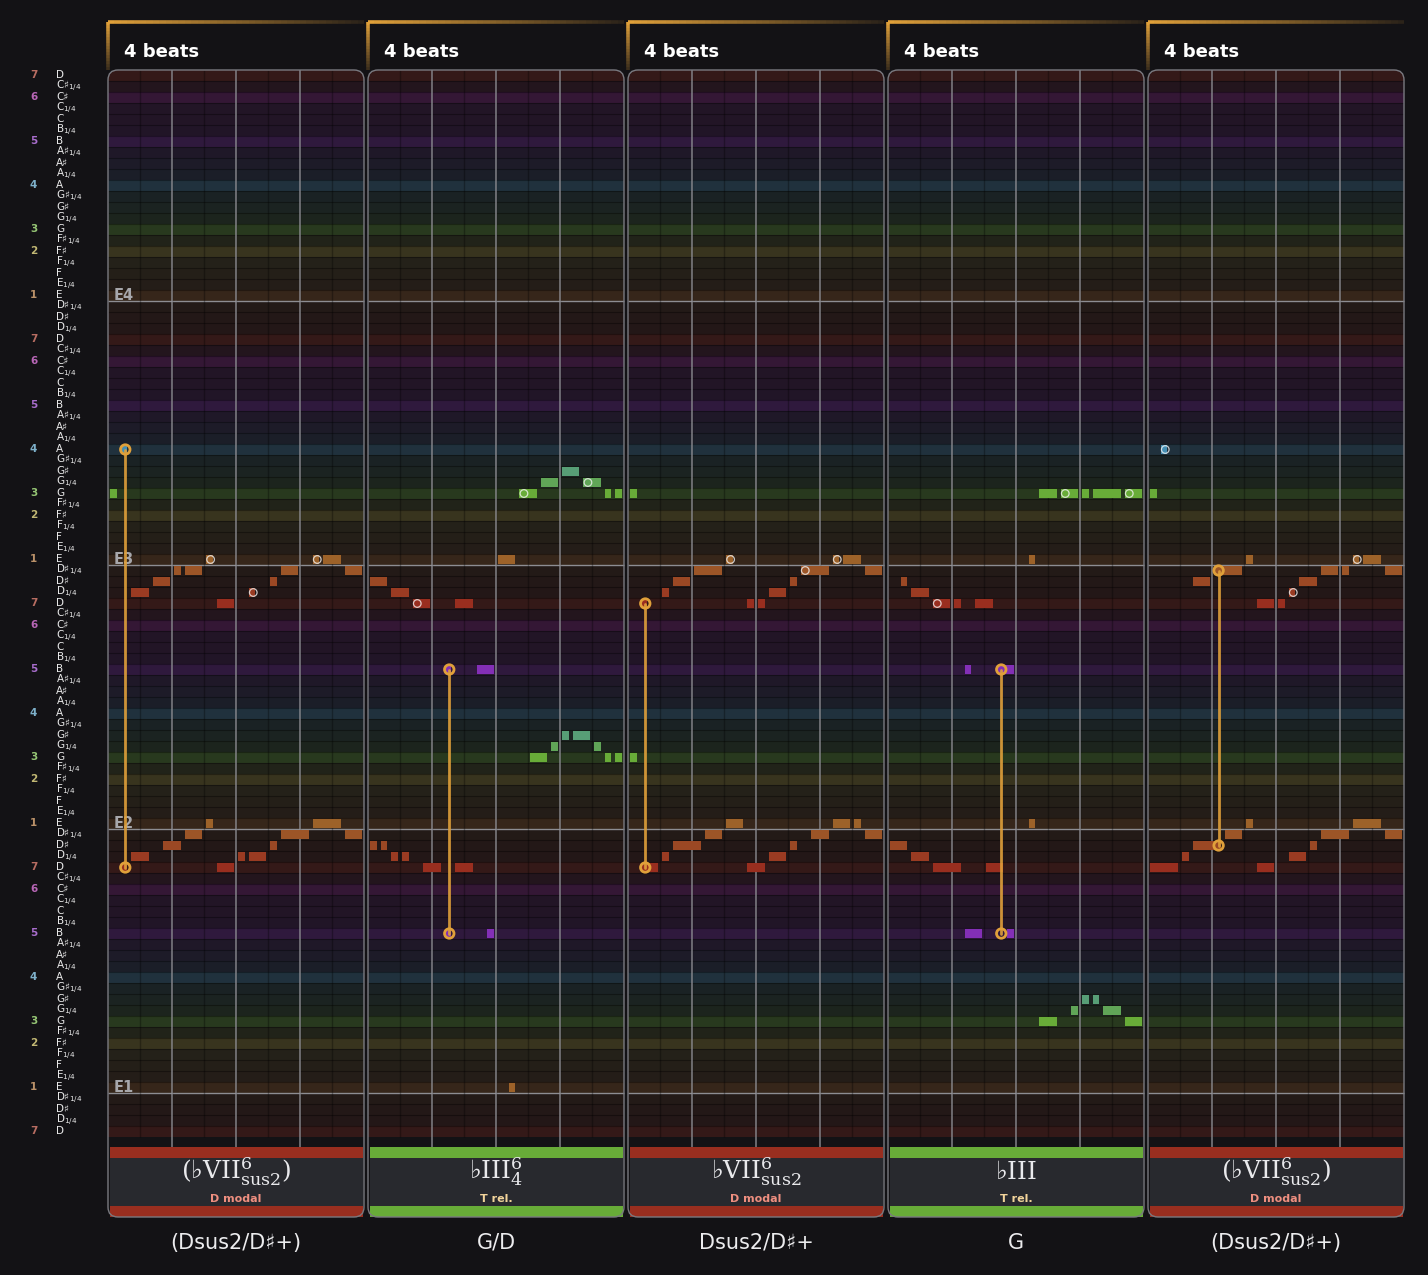
\includegraphics[width=0.85\textwidth]{g_tabroll_armonia_sarniezz.png}
  \caption{Tabroll con armonía (Sarniezz). Arriba, las notas en 24-EDO; debajo de cada compás, el acorde leído: grado, calidad, función y nombre. «Beats»: pulsos del compás.}\label{fig:tabroll-armonia}
\end{figure}

\subsection{Centro, modo y funciones}

\paragraph{Centro.} \texttt{center24\_by\_layer} calcula en cada capa tres repartos sobre las 24 clases: el tiempo que
suena cada clase ($T$), cuántas veces abre o cierra una vuelta del ciclo ($B$) y cuántas veces vuelve después de al menos
dos notas distintas ($R$). Cada reparto se normaliza a suma 1 y el puntaje de la capa es su promedio,
$\tfrac13 (T + B + R)$. El puntaje de la canción pesa el bajo el doble:
\[
  Z = \frac{2 Z^{\mathrm{bajo}} + Z^{\mathrm{aguda}}}{3}, \qquad
  \text{margen} = \frac{Z_{(1)} - Z_{(2)}}{Z_{(1)}},
\]
donde $Z_{(1)}$ y $Z_{(2)}$ son los dos mayores. Un margen menor que 0.1 marca un centro dudoso.

\paragraph{Modo.} \texttt{mode24} suma los perfiles de los compases confiables (bajo con peso 1 y voz aguda con 0.6),
los cuenta desde el centro y, para cada uno de los grados 2, 3, 6 y 7, elige entre su versión rebajada, neutra o natural
la que más suena.

\paragraph{Funciones y progresiones.} \texttt{chord\_roles} cifra cada acorde en números romanos y le asigna función,
eje e inversión (sección~\ref{sec:armonia-teoria}); \texttt{chord\_progressions} clasifica cada cambio de fundamental entre
compases confiables y cuenta las progresiones más frecuentes y los \emph{vaivenes}, idas y vueltas entre dos acordes.

\subsection{Columnas melódicas}

\texttt{melodic\_columns} elige, en cada pulso, la nota de la voz aguda más importante, a la manera de la reducción de
\citet{lerdahl1983}. Cada nota recibe el peso
\[
  \omega = 0.30\, \mu + 0.35\, \alpha + 0.20 \min\{1, d/\text{pulso}\} + 0.15\, \chi,
\]
donde $\mu$ es la posición métrica del ataque (primer pulso 1, mitad del compás 0.85, otro pulso 0.7, corchea 0.45, resto
0.3), $\alpha$ indica si la nota pertenece al acorde (1; a un cuarto de tono, 0.7; fuera, 0.2), $d$ es su duración y
$\chi$ si es un punto alto o bajo del contorno. La nota de más peso del compás, junto con el bajo que suena en ese
momento, es la \emph{columna principal}, que el tabroll marca con anillos dorados.

\section{Mejorar la melodía: hipótesis que se prueban}\label{sec:melodia-hipotesis}

Para mejorar la melodía se probaron varias ideas. Cada cambio se midió en las tres canciones con referencia y solo se
adoptaba si mejoraba en las tres (tabla~\ref{tab:hipotesis}).

\begin{table}[ht]
  \centering\small
  \caption{Ideas probadas para mejorar la melodía.}\label{tab:hipotesis}
  \begin{tabularx}{\textwidth}{@{}>{\raggedright}p{4.6cm}>{\raggedright}X l@{}}
    \toprule
    Idea & Qué pasó & Estado \\
    \midrule
    Consenso entre vueltas del looper & Más rápido y más estable & adoptada \\
    Atracción al registro de la melodía & Mata Zyklek pasa de 57 a 64 & adoptada \\
    Quitar notas sueltas & $+3$ puntos en las tres canciones & adoptada \\
    Guiarse por la partitura & La herramienta debe servir sin partitura; además no mejoraba de forma estable & descartada \\
    REPET (separar lo que se repite) & Solo deja en primer plano entre el 1 y el 18\,\% de la melodía & descartada \\
    Elegir la capa más nueva del looper & Funciona sobre la partitura, falla sobre el audio & descartada \\
    Estéreo por canal & La melodía sigue tapada en el 50--65\,\% de los cuadros & descartada \\
    Basic Pitch & Encuentra menos melodía y no da cuartos de tono & descartada \\
    Unir notas iguales seguidas & Borra re-ataques reales & descartada \\
    Votar la altura entre vueltas, refinar por armónicos, prueba de octava, otros umbrales & Ninguna mejora las tres
    canciones a la vez & descartadas \\
    Bajar el piso de la voz aguda & Empeora las tres canciones & descartada \\
    \bottomrule
  \end{tabularx}
\end{table}

\paragraph{Notas sueltas.} Por cada nota de la melodía principal, la herramienta detectaba 1.3 a 1.5 notas: unas eran de
otras capas del looper y la mayoría, pedazos cortos de una nota partida en cada ataque o cambio de altura. La regla
adoptada quita las notas de menos de 80~ms que no reaparecen a la misma altura una vuelta antes y una vuelta después;
entre esas notas solo el 6 a 24\,\% eran aciertos. La melodía principal pasó de 63.7 a 66.8 en Mata Zyklek, de 43.4 a
46.2 en Sarniezz y de 44.0 a 45.4 en Fabienk; el bajo, de 78.7 a 82.9, de 75.3 a 78.7 y de 63.8 a 69.3.

\paragraph{El looper y la melodía.} REPET \citep{rafii2013} aplicado a la vuelta del looper no sirve: la melodía se
repite en cada vuelta igual que el riff. Elegir la capa más nueva funcionaría con una transcripción perfecta, pero sobre
el audio la melodía aparece entre los picos de un cuadro suelto solo en el 32--43\,\% de los cuadros; la herramienta la
recupera mejor (44--68\,\%) porque promedia vueltas. La conclusión es que el looper ayuda a recuperar la melodía
promediando vueltas, no a separarla.

\paragraph{Basic Pitch.} Con el ajuste de notas cortas, Basic Pitch \citep{bittner2022} encuentra el 36, 47 y 48\,\% de
la melodía (Sarniezz, Mata Zyklek y Fabienk), menos que la herramienta (51, 69 y 49\,\%). Combinado con ella recupera
7--14 puntos más, pero esas notas caen sobre todo donde la herramienta ya tiene otra altura, y ninguna regla para
juntarlas mejora la medida principal. Su salida, en notas MIDI enteras, no sirve para cuartos de tono.

\section{Separar instrumentos}\label{sec:separacion}

La separación por defecto es Demucs \texttt{htdemucs\_6s} \citep{rouard2023}. Como alternativa se integró BS-RoFormer SW
\citep{lu2024}, que en las métricas públicas separa mejor la guitarra (SDR de 9.05 frente a 5.22~dB). El SDR
(\emph{signal-to-distortion ratio}) mide qué tan limpia sale una pista separada frente a la grabada por aparte. La
comparación se hizo sobre Sarniezz con la misma versión del cuaderno y los mismos ajustes; solo cambiaron las pistas. Para
que fuera reproducible se fijaron la versión de la herramienta de separación, el remuestreo, el solapamiento, la
precisión numérica, el número de hilos y la semilla, y se registró la huella SHA-256 del modelo. El resultado está en la
sección~\ref{sec:res-separacion}.

\section{La armonía por compás}\label{sec:armonia-metodo}

\paragraph{Entradas.} Para cada compás se usan el bajo y el contenido de la voz aguda en las 24 clases, sin contar las
notas de menos de un cuarto de pulso, que suelen ser de paso o adornos. El perfil de cada compás se suma sobre todas las
vueltas del ciclo que lo contiene, tomando el mismo punto del ciclo en cada vuelta; el bajo y la voz aguda usan sus
propios ciclos, porque pueden tener periodos distintos.

\paragraph{Acorde.} El perfil se compara con las ocho calidades de la tabla~\ref{tab:calidades}: cuenta lo que cae dentro
del acorde, resta lo que cae fuera y premia que el bajo esté en la fundamental, con peso 1 para el bajo y 0.6 para la voz
aguda.

\paragraph{Confianza.} La confianza $\kappa \in [0, 1]$ es el producto de tres factores: la probabilidad de la
fundamental elegida frente a las otras 23, el acuerdo entre las vueltas del ciclo en ese compás y la cobertura (qué parte
del compás tiene notas). Un compás es confiable si $\kappa \ge 0.5$. En canciones sin looper, como las de Primus, los
compases fuera de ciclo no se castigan.

\paragraph{Centro.} Se adapta la medida en tres partes de Piston para música sin dominante. En cada capa (bajo y voz
aguda) se suman, con el mismo peso, la nota que más tiempo suena, la que más aparece al principio y al final de cada vuelta
y la que más vuelve después de alejarse; el bajo pesa el doble. Elegir el centro solo por el bajo se descartó, porque en
Sarniezz y Fabienk el bajo descansa en \fl VII. El centro usado coincide con la tónica de oído en las cinco canciones
evaluadas (Mata Zyklek Sol, Sarniezz Mi, Fabienk Mi, Utzp Mi, Yor Zarad Sol).

\paragraph{Grado, función y progresión.} Cada acorde se cifra en números romanos sobre el centro, con «+» para el cuarto
de tono y «n» para la tercera neutra, y recibe su función (sección~\ref{sec:armonia-teoria}) y su eje de Lendvai. Cada
cambio de fundamental entre compases confiables se clasifica según el movimiento de la fundamental en la tabla de Piston
(quinta abajo, quinta arriba, tercera, segunda, tritono o microtonal) y según el eje (adelante, atrás, dentro del mismo
eje, en el mismo eje neutro o microtonal).

\section{Evaluación}\label{sec:evaluacion}

\paragraph{Medidas.} Se usa la medida F de notas, con el ataque a $\pm75$~ms y la altura en la misma casilla de 24-EDO.
Se mide para tres referencias: la \emph{melodía principal} de cada sección, elegida por el autor por criterio musical
(la voz que uno cantaría) y nunca mirando qué guitarra sigue la herramienta; la \emph{nota más aguda} de todas las
guitarras, más exigente; y el \emph{bajo}. Las versiones «sin octava» aceptan la misma clase en cualquier octava. Para la
armonía se mide la fundamental por compás, ponderada por su duración, en todos los compases y en los confiables.

\paragraph{Alineación.} El camino entre la partitura y el audio se obtiene por alineamiento temporal dinámico (DTW) y se
ajusta a una recta por sección, porque con looper el tempo no cambia dentro de una sección. Las ventanas incompatibles con
un tempo constante quedan fuera. Este criterio usa solo la alineación, nunca la salida de la herramienta. Se mide el 83\,\%
del tiempo de Mata Zyklek, el 83\,\% de Sarniezz y el 72\,\% de Fabienk.

\paragraph{Arbitraje a ciegas.} Donde la herramienta y la partitura corregida dan alturas distintas una y otra vez, el
autor juzgó de oído, sin saber cuál era cuál. Cada clip tiene la pista de guitarra real en un canal y la partitura
sintetizada en el otro, en tres versiones en orden al azar: la nota escrita, un cuarto de tono arriba y un cuarto de tono
abajo. La regla se fijó antes de escuchar: una nota cambia si al menos dos clips eligen la misma altura distinta de la
partitura, con seguridad media o alta. En la primera ronda (21 clips, 3 de ellos controles, todos correctos) la partitura
tenía razón en la mitad de los casos decididos: un desacuerdo no basta para corregirla, porque la herramienta también se
equivoca en cuartos de tono. La segunda ronda (21 clips) corrigió tres notas de Sarniezz, una pista de Fabienk y añadió
una nota de Mata Zyklek.

\paragraph{Prueba ciega.} Yor Zarad se reservó sin abrir ninguna salida de la herramienta, y su referencia se armó a
ciegas (sección~\ref{sec:referencias}). La medida se hizo una sola vez, sobre la corrida congelada.

\paragraph{Reproducibilidad.} Con las mismas pistas, la herramienta da el mismo resultado: entre 8 y 12 corridas por
canción dieron las mismas notas, la misma F y la misma tabla por compás. Demucs era el único paso al azar (desplaza el
audio entre 0 y 0.5~s antes de separar): con el mismo código, Mata Zyklek dio 57.2 con unas pistas y 61.6 con otras.
Desde entonces la semilla queda fija, y cada corrida guarda la huella SHA-256 \citep{nist2015} de la mezcla y de las dos
pistas, de modo que dos corridas con las mismas huellas usaron exactamente el mismo audio. Un hallazgo solo cuenta si se
mantiene con las dos separaciones. Ninguna celda del cuaderno lee la partitura ni nombra una canción.

\section{Comparación con estilos}\label{sec:comparacion}

\subsection{Matriz de verosimilitud armónica}

Cada estilo se resume por el centro de su corpus en dos cosas: qué fundamentales suenan y cuánto tiempo (12 grados
respecto de la tónica) y cómo se cambia de fundamental (intervalo del cambio y grado de llegada, $12 \times 12$). La
verosimilitud de una canción en un estilo es el percentil de tipicidad respecto del centro, promediado entre esas dos
partes; con menos de tres cambios de acorde, solo cuenta la de las fundamentales. Las fundamentales de la canción se
toman de los compases confiables.

La figura~\ref{fig:matriz-rock-pop} muestra la forma del resultado con los dos estilos más cercanos, rock y pop. Cada
celda es un percentil: 50 es una pieza típica del estilo y 0, una más rara que todas las del corpus.

\begin{figure}[htbp]
  \centering
  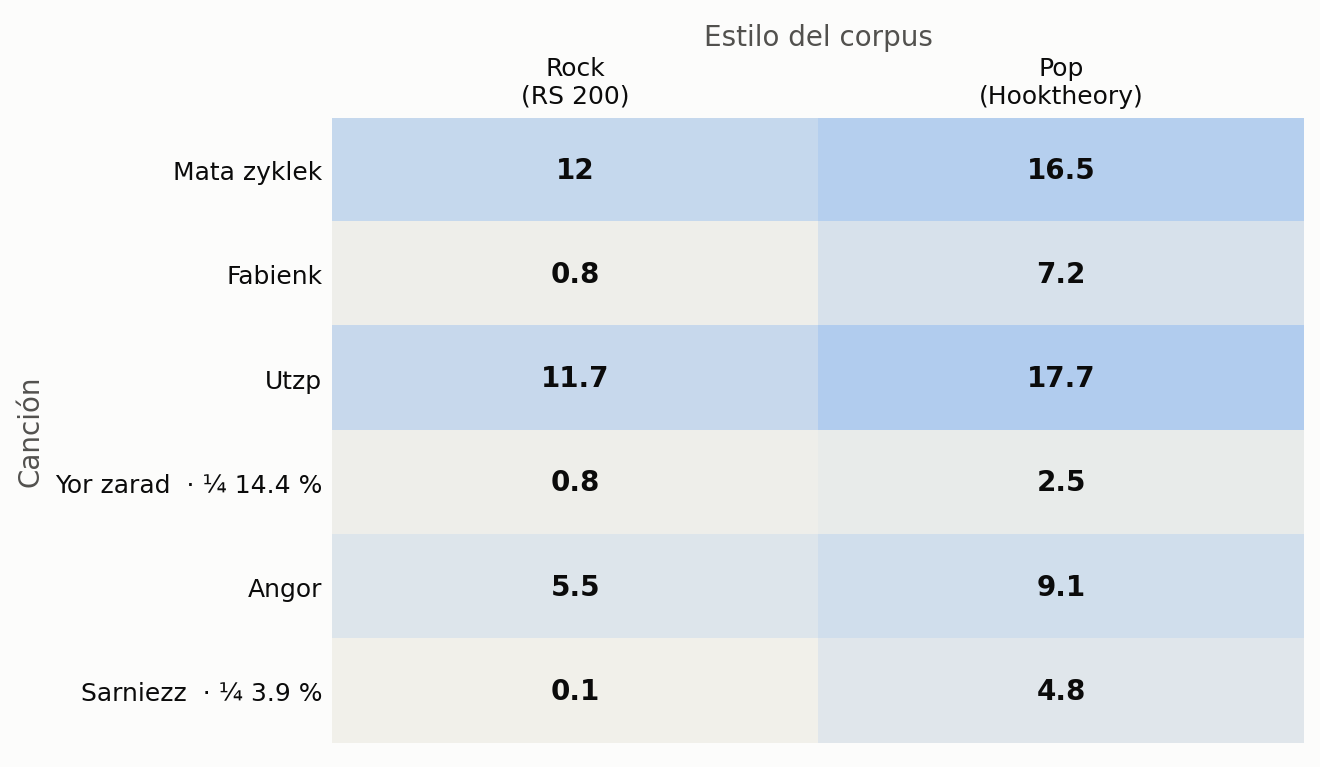
\includegraphics[width=0.6\textwidth]{g_matriz_rock_pop.png}
  \caption{Matriz de verosimilitud frente a rock (RS~200) y pop (Hooktheory). Cada celda es un percentil: 50 = típica del estilo; 0 = más rara que todo el corpus. Junto al nombre, el tiempo con la fundamental en cuarto de tono.}\label{fig:matriz-rock-pop}
\end{figure}

\subsection{Test por bloques}

Cada canción se resume en cuatro bloques de rasgos, y cada bloque se compara con cada corpus que lo tenga:
\begin{itemize}
  \item \textbf{Armonía:} fundamentales y cambios de fundamental, como en la matriz.
  \item \textbf{Escala (12 notas):} la melodía en 12 grados respecto de la tónica, por duración; cada cuarto de tono se
  reparte mitad y mitad entre sus dos vecinos.
  \item \textbf{Cuartos de tono:} el reparto del tiempo entre los 12 grados en cuarto de tono, comparado solo con los
  corpus microtonales.
  \item \textbf{Metro:} el reparto del tiempo por familia de compás (2·4·8, 3·6·12, 5, 7, 9 u otro impar).
\end{itemize}

La tipicidad de un bloque se mide con el percentil por vecinos ($k = 5$). Una canción solo pasa al bloque de cuartos de
tono si la concentración de sus cuartos de tono (sección~\ref{sec:metodo-cuartos}) supera a la de los controles por al
menos dos desviaciones estándar; si no, se trata como una canción de 12 notas.

\paragraph{Modelo de medición.} La herramienta marca entre 9 y 13\,\% de cuartos de tono en música que no los tiene y lee
mal algunos compases de un 4/4. Para comparar en igualdad, cada pieza de corpus pasa por el mismo error: en la altura, una
fracción $\varepsilon$ del tiempo de cada grado se reparte entre sus dos vecinos a un cuarto de tono; en el metro, una
fracción $\eta$ pasa a las familias de compás en que la herramienta se equivoca. Ambas se miden en los controles de
Primus ($\varepsilon = 0.113$).

\paragraph{Veredicto.} Con un umbral $u = 5$\,\%, como un contraste a una cola:
\begin{itemize}
  \item \emph{estilo existente (X)}: algún corpus X con todos los bloques medidos tiene percentil conjunto $\ge u$;
  \item \emph{variante atípica de X}: cada bloque es típico en X por separado, pero la combinación no lo es;
  \item \emph{síntesis de lenguajes existentes}: cada bloque es típico en algún corpus, pero ningún corpus explica la
  combinación;
  \item \emph{rasgo sin vecino}: algún bloque no es típico en ningún corpus.
\end{itemize}
El percentil conjunto mide el parecido en todos los bloques a la vez, con la suma de las distancias de cada bloque
divididas por su mediana en el corpus. Solo cuentan los corpus con 100 piezas o más.

\paragraph{Calibración.} El mismo veredicto se aplica a cada pieza de los corpus con al menos tres bloques, contra las
demás, para saber cuántas veces el método llama «síntesis» o «sin vecino» a una pieza real de un estilo conocido.

\section{Cuartos de tono: adorno o grado}\label{sec:metodo-cuartos}

Cada nota en cuarto de tono de la voz aguda se clasifica como \emph{inflexión} (adorno) si dura menos que la nota mediana
de la canción y llega o sale por un paso de cuarto de tono hacia un grado regular (un bend, un slide, una nota de paso), y
como \emph{grado} en cualquier otro caso. La \emph{concentración} es el porcentaje del tiempo en cuartos de tono que cae
en los dos grados más usados: si es alta, los cuartos de tono son grados elegidos de la escala; si se reparten por igual
entre muchos grados, son desafinación o adorno. Para cada grado en cuarto de tono se mide además en qué porcentaje de las
vueltas del ciclo principal aparece.

El \emph{piso de ruido} se mide en Primus: la herramienta marca allí entre el 9 y el 13\,\% de la melodía en cuartos de
tono, casi todo como inflexión. La proporción de tiempo en cuartos de tono no sirve para separar a la banda (Utzp marca
11\,\%), pero la concentración sí: en Primus está entre 28 y 37\,\%.

\section{Ciclos métricos}

La herramienta parte la canción en compases de 2 a 8 pulsos, así que un ciclo más largo sale partido en trozos (por
ejemplo $4 + 4 + 4 + 7$). Para encontrar los ciclos largos se calcula $R(\ell)$ en una rejilla de corcheas, para $\ell$
de 2 a 40, en toda la canción y en ventanas de 30~s. Además se listan los tramos seguidos de compases con el mismo número
de pulsos y se buscan patrones de compases que se repiten.

\section{Implementación}

El cuaderno de Jupyter es la fuente de verdad del análisis. Un script lo divide en un módulo por celda y guarda la huella
de cada uno; si un módulo se edita a mano, la extracción se detiene en lugar de borrar el cambio. Otro script corre todas
las celdas sobre una canción, de punta a punta, y guarda el tabroll, la armonía, los ciclos y un resumen con las huellas
del audio usado. El repositorio incluye las referencias, la documentación, las pruebas automáticas y la presentación. Está
escrito en Python con \texttt{librosa} \citep{mcfee2015}. El código es público en
\url{https://github.com/NewForest2005/analisis-computacional-tabroll}.
